\documentclass[border=3pt,tikz]{standalone}
% Shared look for every TikZ figure in these notes.
% Included by each standalone figure file; also keeps the figures consistent
% with the colours used in the PDF and on the website.

\usepackage{tikz}
\usepackage{pgfplots}
\pgfplotsset{compat=1.18}
\usetikzlibrary{arrows.meta, decorations.markings, decorations.pathmorphing,
                patterns, calc, positioning}
\usepackage{amsmath}

% Series colours are the three validated categorical slots also used by the
% interactive widgets, so a path drawn in the printed notes and the same path on
% the website are the same colour. They clear the colour-vision-deficiency and
% contrast checks as a set; every path is direct-labelled as well, so colour is
% never the only thing carrying identity.
\definecolor{duPurple}{HTML}{68246D}
\definecolor{duBlue}{HTML}{2A78D6}
\definecolor{duRed}{HTML}{EB6834}
\definecolor{duGreen}{HTML}{1BAF7A}
\definecolor{duGrey}{HTML}{4D4D4D}

\tikzset{
  % heavier default lines and arrow tips, so diagrams stay clear when zoomed
  every picture/.append style = {line width=0.7pt, >={Stealth[length=3mm]}},
  axisline/.style   = {-{Stealth[length=3.4mm]}, line width=1.0pt, black},
  path1/.style      = {duBlue,   line width=1.6pt},
  path2/.style      = {duRed,    line width=1.6pt},
  path3/.style      = {duGreen,  line width=1.6pt},
  statedot/.style   = {circle, fill=black, inner sep=1.8pt},
  arrowhead/.style  = {decoration={markings,
                        mark=at position #1 with {\arrow{Stealth[length=3.4mm]}}},
                       postaction={decorate}},
  lbl/.style        = {font=\normalsize},
  slbl/.style       = {font=\small, duGrey},
  workfill/.style   = {duPurple, opacity=0.16},
}

% larger labels in plots as well
\pgfplotsset{every axis/.append style={label style={font=\normalsize}, tick label style={font=\small}, line width=0.9pt}}

% Closed system: a piston-cylinder going from state 1 to state 2.
\begin{document}
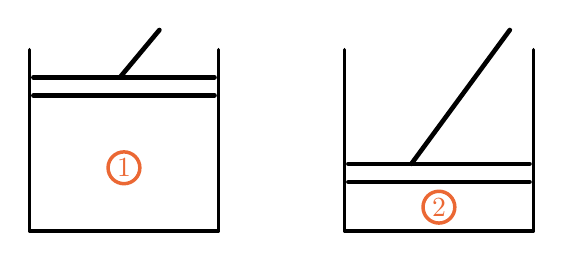
\begin{tikzpicture}[x=1cm, y=1cm,
    wall/.style={line width=1.3pt, line join=round, line cap=round},
    piston/.style={line width=1.68pt, line cap=round},
    state/.style={circle, draw=duRed, text=duRed, line width=1.26pt,
                  inner sep=1.2pt, font=\normalsize}]
  % state 1: piston near the top
  \draw[wall] (0,2.3) -- (0,0) -- (2.4,0) -- (2.4,2.3);
  \draw[piston] (0.05,1.95) -- (2.35,1.95);
  \draw[piston] (0.05,1.72) -- (2.35,1.72);
  \draw[piston] (1.15,1.95) -- (1.65,2.55);
  \node[state] at (1.2,0.8) {1};
  % state 2: piston pushed down
  \begin{scope}[xshift=4cm]
    \draw[wall] (0,2.3) -- (0,0) -- (2.4,0) -- (2.4,2.3);
    \draw[piston] (0.05,0.85) -- (2.35,0.85);
    \draw[piston] (0.05,0.62) -- (2.35,0.62);
    \draw[piston] (0.85,0.85) -- (2.1,2.55);
    \node[state] at (1.2,0.3) {2};
  \end{scope}
\end{tikzpicture}
\end{document}
